% Figure 5 in the source manuscript, Figure 4 in this blog post.
% The original title reverses the colour key. Hide that title in the document
% using graphicx layout cropping; retain the original image and numerical data.
% Source PNG is 100 dpi: 34.56 bp trims 48 pixels from its top margin.
\begin{figure}[H]
    \centering
    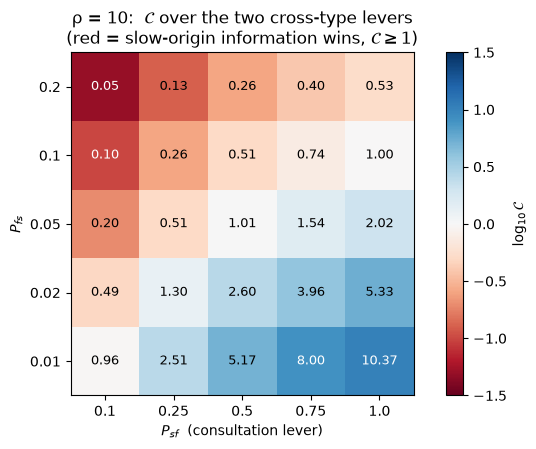
\includegraphics[trim=0 0 0 34.56bp,clip,width=0.78\linewidth]{images/joint-probability-balance.png}
    \caption{Joint variation of $P_{sf}$ and $P_{fs}$ at $\rho=10$, with $P_{ff}=P_{ss}=0.1$. Cell labels show numerical estimates of $C$, while colours show $\log_{10}C$: blue indicates $C>1$, red indicates $C<1$, and white is near balance. The mean-field balance condition is $P_{sf}=10P_{fs}$.}
    \label{fig:joint-probability-balance}
\end{figure}
